\documentclass[10pt]{scrartcl}
\usepackage{geometry}
\usepackage[parfill]{parskip}
\usepackage{graphicx}
\usepackage{amssymb}
\usepackage{epstopdf}
\usepackage{color}
\usepackage{tikz}
\usetikzlibrary{positioning}
\usetikzlibrary{arrows,automata}

\usepackage{listings}

\lstdefinelanguage{FSharp}%
{morekeywords={let, new, match, with, rec, open, module, namespace, type, of, member, %
and, for, while, true, false, in, do, begin, end, fun, function, return, yield, try, %
mutable, if, then, else, cloud, async, static, use, abstract, interface, inherit, finally },
otherkeywords={ let!, return!, do!, yield!, use!, var, from, select, where, order, by },
keywordstyle=\color{bluekeywords},
sensitive=true,
basicstyle=\ttfamily,
breaklines=true,
xleftmargin=\parindent,
aboveskip=\bigskipamount,
tabsize=4,
morecomment=[l][\color{greencomments}]{///},
morecomment=[l][\color{greencomments}]{//},
morecomment=[s][\color{greencomments}]{{(*}{*)}},
morestring=[b]",
showstringspaces=false,
literate={`}{\`}1,
stringstyle=\color{redstrings},
} 

\lstset{
  frame=single,language=FSharp,
   basicstyle=\footnotesize,
  escapechar=\@,
  basicstyle=\footnotesize, frame=tb,
  numbers=left,
  stepnumber=2,
  numbersep=5pt, 
  numberstyle=\tiny\color{mygray},
  xleftmargin=.2\textwidth, xrightmargin=.2\textwidth
}
\usepackage{geometry}
 \geometry{
 a4paper,
 total={210mm,297mm},
 left=20mm,
 right=20mm,
 top=20mm,
 bottom=20mm,
 }
\definecolor{bluekeywords}{rgb}{0.13,0.13,1}
\definecolor{greencomments}{rgb}{0,0.5,0}
\definecolor{redstrings}{rgb}{0.9,0,0}
\definecolor{mygray}{rgb}{0.2,0.2,0.2}

\DeclareGraphicsRule{.tif}{png}{.png}{`convert #1 `dirname #1`/`basename #1 .tif`.png}

\title{02257 - Applied functional programming}
\subtitle{Project 3 - A game with a graphical user interface}
\author{Anna Maria Walach - \textit {s121540@student.dtu.dk} \\ Kim Rostgaard Christensen - \textit {s084283@student.dtu.dk}}
\begin{document}
\maketitle
\section{Type declarations}
\begin{lstlisting}
type NimGameState = State of List<int>
type NimPlayer    = AI | Human
type NimGame      = Nim of State * NimPlayer
\end{lstlisting}

\begin{lstlisting}
type NimGameUI
type NimLancher
\end{lstlisting}

\section{Signatures of the main functions}


\section{Structure overview}
We've divided the user interface of the game into two larger components; the launcher and the game itself. The launcher handles download of games and may bootstrap the a game user interface with a downloaded game configuration.
\subsection{Modules}
The application contains 5 modules:
\begin{itemize}
\item \texttt{NimMain} - starting point for the whole application,
\item \texttt{NimLauncher} - module responsible for handling the logic of download game window,
\item \texttt{NimGame} - module responsible for handling the logic of the game
\item \texttt{NimGUI} - module, that stores, updates and creates almost all GUI elements for \texttt{NimLauncher} and \texttt{NimGame}.
\item \texttt{NimAI} - small modules that stores and provide functions to generate the AI move
\end{itemize}
\subsection{Finite automaton}
\begin{center}
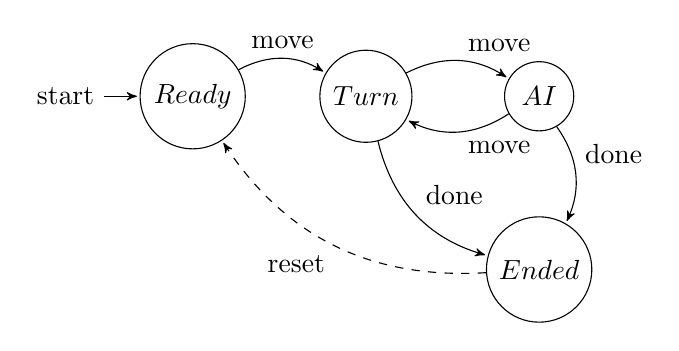
\begin{tikzpicture}[>=stealth',shorten >=1pt,auto,node distance=2.2cm]
  \node[initial,state] (Ready)           {$Ready$};
  \node[state]         (Turn)     [right of=Ready]  {$Turn$};
  \node[state]         (AI)       [right of=Turn]   {$AI$};
  \node[state]         (Ended) [below of=AI]     {$Ended$};


  \path[->]
     (Ready) edge [bend left]  node {move} (Turn)
      (Turn) edge [bend left]  node {move} (AI)
        (AI) edge [bend left]  node {done} (Ended)
        (AI) edge [bend left]  node {move} (Turn)
      (Turn) edge [bend right] node {done} (Ended);
  \path[->, dashed]
      (Ended) edge [bend left] node {reset} (Ready); 
\end{tikzpicture}
\end{center}
The reset signal may, technically speaking, be sent from every state but is left out of the diagram to avoid clutter.
\begin{center}
%type Message =
%  | Download of string * Control * Control| Cancel | Web of string | Error | Cancelled 


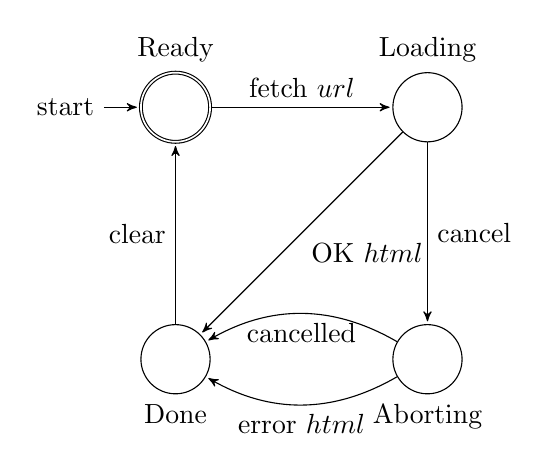
\begin{tikzpicture}[>=stealth',shorten >=1pt,auto,node distance=3.2cm]
  \node[initial,state,accepting,label=above:Ready] (Ready)                       {};
  \node[state,label=above:Loading]                   (Loading)  [right of=Ready]   {};
  \node[state,label=below:Aborting]                   (Aborting) [below of=Loading] {};
  \node[state,label=below:Done]                   (Done)     [below of=Ready]   {};

  \path[->]
        (Ready) edge              node {fetch $url$}  (Loading)
      (Loading) edge              node {cancel}       (Aborting)
     (Aborting) edge [bend left]  node {error $html$} (Done)
     (Aborting) edge [bend right] node {cancelled}    (Done)
      (Loading) edge              node {OK $html$}    (Done);
  \path[->,label]
         (Done) edge              node {clear}        (Ready); 
\end{tikzpicture}
\end{center}

\section{Extensions}
We've extended the basic solution with a more accurate graphical representation of the heaps.	
\begin{center}
\includegraphics[width=0.5\textwidth]{game_ui}
\end{center}

\section{Conclusions}
\bibliographystyle{plain}
\bibliography{references}

\end{document}  
